\documentclass[conference]{IEEEtran}
\IEEEoverridecommandlockouts

\usepackage{cite}
\usepackage{amsmath,amssymb,amsfonts}
\usepackage{graphicx}
\usepackage{textcomp}
\usepackage{xcolor}
\usepackage{booktabs}
\usepackage{multirow}
\usepackage{algorithm}
\usepackage{algorithmic}
\usepackage{tikz}
\usetikzlibrary{positioning, arrows.meta, fit, backgrounds}
\usepackage{hyperref}

\def\BibTeX{{\rm B\kern-.05em{\sc i\kern-.025em b}\kern-.08em
    T\kern-.1667em\lower.7ex\hbox{E}\kern-.125emX}}

\begin{document}

\title{Multi-Task Learning for Simultaneous Instance Segmentation\\
and Pose Estimation of Laboratory Mice}

\author{
  \IEEEauthorblockN{Thanabat Sriphrom}
  \IEEEauthorblockA{
    \textit{Department of Computer Engineering}\\
    \textit{[University Name]}\\
    Bangkok, Thailand\\
    thanabat.srp@gmail.com
  }
}

\maketitle

% ------------------------------------------------------------------
\begin{abstract}
Automated behavioral analysis of laboratory mice is essential for
preclinical drug evaluation, yet existing pose estimation and
segmentation tools operate as separate pipelines requiring manual
integration. We propose \textbf{HybridMTLNet}, a multi-task learning
framework that simultaneously performs instance segmentation and
keypoint estimation for up to two mice in a single forward pass,
without requiring bounding-box annotations. The architecture comprises
a shared ResNet-34 encoder, a U-Net segmentation decoder, and a
deconvolutional pose head. Instance ambiguity is resolved at training
time via Hungarian matching on mask IoU, enabling order-invariant
learning. Evaluated on a dataset of 4{,}000 images spanning eight
behavioral test paradigms, HybridMTLNet attains 0.8090 mIoU and
0.9664 PCK@0.05, matching or exceeding dedicated single-task
baselines (YOLO26, Mask R-CNN, and DeepLabCut) while producing both
outputs in a single forward pass at roughly half the parameters and
compute of an equivalent two-model pipeline.
\end{abstract}

\begin{IEEEkeywords}
multi-task learning, pose estimation, instance segmentation,
laboratory mice, behavioral analysis, Gaussian heatmap
\end{IEEEkeywords}

% ------------------------------------------------------------------
\section{Introduction}

Behavioral phenotyping of laboratory mice is a cornerstone of
preclinical neuroscience and pharmacology. Tasks such as Y-maze
exploration, mirror-box interaction, and forced swim tests are
routinely used to assess the efficacy of novel drug candidates.
Traditional tracking systems, such as ANY-maze and EthoVision XT,
rely on color-based blob detection or physical markers attached to
the animal, both of which fail under occlusion, varying illumination,
or multi-animal interaction, and may alter natural behavior
\cite{mathis2018deeplabcut}.

Deep learning has advanced markerless animal pose estimation
significantly, most notably through DeepLabCut \cite{mathis2018deeplabcut}
and SLEAP \cite{pereira2022sleap}. However, these systems treat pose
estimation and body segmentation as independent tasks, requiring
separate models and post-hoc integration. Object detection frameworks
such as YOLO26 \cite{jocher2023ultralytics} offer unified detection
and segmentation or pose estimation, but again in separate model
variants rather than a single unified representation.

We address this gap by proposing \textbf{HybridMTLNet}, a hybrid
multi-task architecture that produces per-instance segmentation masks
and Gaussian keypoint heatmaps from a single shared encoder.
The key contributions of this work are:

\begin{itemize}
  \item A unified architecture for simultaneous instance segmentation
        and pose estimation without bounding-box supervision.
  \item An order-invariant training scheme via Hungarian matching on
        mask IoU, enabling robust multi-instance learning.
  \item Comprehensive evaluation across eight behavioral paradigms
        demonstrating consistent superiority over single-task baselines.
\end{itemize}

% ------------------------------------------------------------------
\section{Related Work}

\subsection{Animal Pose Estimation}
Mathis et al.\ introduced DeepLabCut \cite{mathis2018deeplabcut},
adapting ResNet-based transfer learning to lab-animal keypoint
detection, establishing Gaussian heatmap regression as the dominant
paradigm for animal pose estimation. SLEAP \cite{pereira2022sleap}
extended this to multi-animal scenarios using part-affinity fields.
Both systems, however, output only skeletal keypoints without body
segmentation.

\subsection{Instance Segmentation}
Mask R-CNN \cite{he2017maskrcnn} established the detect-then-segment
paradigm, while more recent one-stage methods such as YOLO26-Seg
\cite{jocher2023ultralytics} achieve real-time instance segmentation
through a lightweight prototype mask head. These methods require
bounding-box annotations and produce segmentation independently of
keypoints.

\subsection{Multi-Task Learning}
Multi-task learning (MTL) exploits shared representations to improve
generalization across related tasks \cite{caruana1997multitask}.
In human pose and segmentation, Parsing R-CNN
\cite{yang2019parsingrcnn} and UniPose \cite{jin2020whole} demonstrate
that joint training improves both tasks.

Several systems combine segmentation and pose estimation for
laboratory animals, but all adopt a \emph{modular pipeline} of
separately trained models rather than a single jointly optimized
network. SIPEC \cite{marks2022sipec} analyzes interacting mice and
primates through four independent modules---a Mask R-CNN segmentation
network, a DenseNet identification network, a pose network, and a
behavior classifier---each trained and run in sequence. STCS
\cite{tang2024stcs} chains segmentation, tracking, and clustering
stages, and like top-down pose pipelines requires bounding-box
annotations. More recently, InteBOMB \cite{zhai2025intebomb}
integrates generic object tracking and segmentation with pose
estimation, but again couples pre-existing models rather than
sharing a representation.

A single-network alternative is YOLO-SP \cite{jiang2025yolosp}, which
extends YOLOv11 with separate segmentation and pose heads to output
both tasks in one pass. It is, however, a detection-based design that
relies on bounding-box proposals, and is developed and evaluated for
agricultural harvesting (bell peppers) rather than laboratory animals.

By contrast, HybridMTLNet employs a box-free, dense-prediction design:
a shared encoder feeds a U-Net segmentation decoder and a
deconvolutional pose head, resolving instances by Hungarian matching
on mask IoU rather than bounding boxes. To our knowledge, it is the
first single-network model to jointly produce instance segmentation
and keypoint estimation for laboratory mice without bounding-box
supervision, rather than composing independently trained models.

% ------------------------------------------------------------------
\section{Methodology}

\subsection{Dataset}
We curate a dataset of 4{,}000 images captured from eight standard
behavioral test paradigms: Y-maze, mirror box, forced swim, open
field, elevated plus maze, rotarod, social interaction, and novel
object recognition. Images contain one or two C57BL/6 mice and are
annotated with per-instance binary segmentation masks and three
skeletal keypoints per animal (nose, shoulder, tail base).
Critically, no bounding-box annotations are required.
Images are split 80\,/\,10\,/\,10 into train, validation, and test sets.
Original image resolution is 640\(\times\)360 pixels; all models
are trained and evaluated at 256\(\times\)256.

\subsection{Architecture}

\begin{figure}[t]
  \centering
  \resizebox{\columnwidth}{!}{%
  \begin{tikzpicture}[
      font=\small,
      box/.style={draw, rounded corners, minimum height=8mm, align=center, inner sep=3pt},
      enc/.style={box, fill=blue!12},
      dec/.style={box, fill=green!12},
      head/.style={box, fill=orange!15},
      out/.style={box, fill=gray!10},
      arr/.style={-{Latex[length=2mm]}, thick},
    ]
    \node[box, fill=gray!8] (in) {Input\\$256{\times}256{\times}3$};
    \node[enc, right=7mm of in] (enc) {ResNet-34\\shared encoder};
    \node[dec, above right=4mm and 9mm of enc] (segdec) {U-Net\\seg decoder};
    \node[head, below right=4mm and 9mm of enc] (posehead) {Deconv\\pose head};
    \node[out, right=7mm of segdec] (segout) {2 masks\\(instances)};
    \node[out, right=7mm of posehead] (poseout) {6 heatmaps\\($3\,\mathrm{kp}{\times}2$)};

    \draw[arr] (in) -- (enc);
    \draw[arr] (enc.east) to[out=30, in=180] (segdec.west);
    \draw[arr] (enc.east) to[out=-30, in=180] (posehead.west);
    \draw[arr] (segdec) -- (segout);
    \draw[arr] (posehead) -- (poseout);

    \begin{scope}[on background layer]
      \node[draw, dashed, rounded corners, fit=(segdec)(segout),
            inner sep=4pt, label=above:{Segmentation}] {};
      \node[draw, dashed, rounded corners, fit=(posehead)(poseout),
            inner sep=4pt, label=below:{Pose}] {};
    \end{scope}
  \end{tikzpicture}%
  }
  \caption{HybridMTLNet architecture. A shared ResNet-34 encoder
  feeds into (1) a U-Net segmentation decoder producing two binary
  instance masks and (2) a deconvolutional pose head producing six
  Gaussian heatmaps (3 keypoints \(\times\) 2 instances).}
  \label{fig:arch}
\end{figure}

HybridMTLNet (Fig.~\ref{fig:arch}) consists of three components:

\noindent\textbf{Shared Encoder.}
A ResNet-34 \cite{he2016resnet} backbone pre-trained on ImageNet
serves as a shared feature extractor. Skip connections at four
resolution levels are preserved for the segmentation decoder.

\noindent\textbf{Segmentation Decoder.}
A U-Net-style decoder \cite{ronneberger2015unet} progressively
upsamples encoder features via bilinear interpolation and skip
connections, producing a two-channel output \(\hat{S} \in
\mathbb{R}^{2 \times H \times W}\), where each channel represents
the binary mask of one mouse instance.

\noindent\textbf{Pose Head.}
Four successive deconvolutional layers upsample the bottleneck
features to produce six Gaussian heatmaps \(\hat{H} \in
\mathbb{R}^{6 \times H \times W}\) (3~keypoints \(\times\)
2~instances). Keypoint coordinates are recovered as the
\(\arg\max\) of each heatmap channel.

\subsection{Loss Function}
The total loss is a weighted sum:
\begin{equation}
  \mathcal{L} = \lambda_{\text{seg}}\,\mathcal{L}_{\text{seg}}
              + \lambda_{\text{pose}}\,\mathcal{L}_{\text{pose}}
  \label{eq:loss}
\end{equation}

The segmentation loss combines binary cross-entropy and Dice loss
\cite{milletari2016vnet}:
\begin{equation}
  \mathcal{L}_{\text{seg}} = \mathcal{L}_{\text{BCE}} +
  \left(1 - \frac{2\sum p\,g}{\sum p + \sum g + \epsilon}\right)
\end{equation}

The pose loss is mean-squared error between predicted and target
Gaussian heatmaps:
\begin{equation}
  \mathcal{L}_{\text{pose}} = \frac{1}{K}
  \sum_{k=1}^{K} \|\hat{H}_k - H_k\|_2^2
\end{equation}

Because MSE on sparse Gaussian maps is naturally two to three orders
of magnitude smaller than BCE+Dice, we set
\(\lambda_{\text{seg}} = 1\) and \(\lambda_{\text{pose}} = 400\)
to balance gradient magnitudes.

\subsection{Order-Invariant Instance Matching}
Since instance ordering is arbitrary, we apply Hungarian matching
\cite{kuhn1955hungarian} at each training step. A cost matrix
\(C \in \mathbb{R}^{N_{\text{pred}} \times N_{\text{gt}}}\) is
constructed using pairwise mask IoU, and the optimal assignment
is solved via the linear sum assignment algorithm. Ground-truth
masks and heatmaps are reordered accordingly before computing
\(\mathcal{L}\).

\subsection{Data Augmentation}
Training images undergo random horizontal flip (p\,=\,0.5),
vertical flip (p\,=\,0.5), rotation \(\pm 30^\circ\)
(p\,=\,0.5), and color jitter (brightness \(\times[0.7,1.3]\),
contrast \(\times[0.8,1.2]\), p\,=\,0.5). All geometric
transformations are applied consistently to images, masks,
and keypoint coordinates.

% ------------------------------------------------------------------
\section{Experiments}

\subsection{Implementation Details}
HybridMTLNet is implemented in PyTorch 2.0. Training uses the
Adam optimizer with initial learning rate \(10^{-4}\), reduced by
0.5$\times$ at epoch 84, for a total of 100 epochs with batch
size 16. YOLO26 baselines use the same 256\(\times\)256
input resolution and 100 training epochs. All experiments are
conducted on a single NVIDIA GPU with at least 6~GB VRAM.

\subsection{Evaluation Metrics}

\noindent\textbf{mIoU.}
Mean Intersection over Union over matched instance pairs:
\begin{equation}
  \text{mIoU} = \frac{1}{N}\sum_{i=1}^{N}
  \frac{|P_i \cap G_i|}{|P_i \cup G_i|}
\end{equation}
Instance pairs are found via Hungarian matching on mask IoU,
consistent with the training objective.

\noindent\textbf{PCK@0.05.}
Percentage of Correct Keypoints with threshold 5\% of image
size (12.8\,px at 256\(\times\)256), following Yang and Ramanan
\cite{yang2013pck} and Mathis et al.\ \cite{mathis2018deeplabcut}.
Invisible keypoints (annotated as origin) are excluded from
the count.

\subsection{Baseline Models}
We compare against four single-task baselines trained on the same split:
\begin{itemize}
  \item \textbf{YOLO26m-Seg}: YOLO26m-seg \cite{jocher2023ultralytics}
        trained for instance segmentation, evaluated on mIoU.
  \item \textbf{Mask R-CNN} \cite{he2017maskrcnn}: ResNet-50-FPN
        instance segmentation model (COCO-pretrained) trained for
        segmentation only, evaluated on mIoU.
  \item \textbf{YOLO26m-Pose}: YOLO26m-pose \cite{jocher2023ultralytics}
        trained for keypoint estimation, evaluated on PCK@0.05.
  \item \textbf{DeepLabCut} (maDLC 2.3) \cite{mathis2018deeplabcut}:
        multi-animal ResNet-50 + PAF model trained for keypoint
        estimation only, evaluated on PCK@0.05.
\end{itemize}
All baselines operate as single-task models and cannot jointly
produce segmentation and pose outputs.

% ------------------------------------------------------------------
\section{Results and Discussion}

\subsection{Quantitative Comparison}

\begin{table}[t]
\caption{Test set performance. Best results in \textbf{bold}.
``—'' indicates the model does not perform that task.}
\label{tab:results}
\centering
\begin{tabular}{lccc}
\toprule
\textbf{Model} & \textbf{Tasks} & \textbf{mIoU} & \textbf{PCK@0.05} \\
\midrule
YOLO26m-Seg          & Seg only  & 0.5451 & —      \\
Mask R-CNN           & Seg only  & 0.7774 & —      \\
YOLO26m-Pose         & Pose only & —      & 0.8872 \\
DeepLabCut (maDLC)   & Pose only & —      & 0.4098 \\
\midrule
\textbf{HybridMTLNet (Ours)} & \textbf{Seg + Pose} & \textbf{0.8090} & \textbf{0.9664} \\
\midrule
\multicolumn{2}{l}{\(\Delta\) vs.\ best single-task} & +0.032 & +0.079 \\
\bottomrule
\end{tabular}
\end{table}

Table~\ref{tab:results} presents results on the held-out test set.
HybridMTLNet achieves 0.8113 mIoU and 0.9621 PCK@0.05, surpassing
the YOLO26m-Seg baseline by \(+0.266\) mIoU (\(+48.8\%\) relative)
and the YOLO26m-Pose baseline by \(+0.075\) PCK (\(+8.4\%\) relative).
DeepLabCut (maDLC), trained as a dedicated pose estimator, achieves
only 0.4098 PCK@0.05, substantially below both YOLO26m-Pose and
HybridMTLNet. This gap arises because maDLC uses part affinity fields
designed for full-body multi-animal tracking rather than compact
three-keypoint topologies, and its inference resolution is mismatched
when evaluated at 256\(\times\)256.

On segmentation, HybridMTLNet (0.8113 mIoU) also surpasses
Mask R-CNN (0.7774 mIoU), a strong COCO-pretrained ResNet-50-FPN
detector. We verified this baseline is trained to convergence: its
validation mIoU saturated within the first few epochs and remained
stable through 100 epochs, so the gap reflects a genuine modelling
difference rather than under-training. We attribute this to the decoder
design: Mask R-CNN predicts each instance mask at a fixed
\(28\times28\) RoI resolution before upsampling, which limits
boundary fidelity at small input sizes, whereas our U-Net decoder
with skip connections produces dense per-pixel masks at the full
\(256\times256\) resolution. Notably, HybridMTLNet achieves this
with fewer parameters (28.7\,M vs.\ 43.9\,M) while additionally
producing pose output in the same forward pass. The advantage over
YOLO26m-Seg follows the same reasoning, as YOLO's prototype mask
head is tuned for \(640\times640\) inputs. We emphasise that this
segmentation gain is architectural rather than a multi-task effect:
as the ablation in Section~\ref{sec:ablation} shows, joint training
yields segmentation accuracy on par with a single-task variant of
the same network, not above it.

On pose estimation, HybridMTLNet reaches 0.9621 PCK@0.05, well
above YOLO26m-Pose (0.8872) and DeepLabCut (0.4098). Crucially,
this is achieved while \emph{simultaneously} producing segmentation
from a single model, rather than requiring a separate dedicated
pose network.

\subsection{Qualitative Results}
Figure~\ref{fig:qualitative} shows HybridMTLNet predictions on one
test image from each of the eight behavioral paradigms. The model
produces per-instance masks (coloured overlays) and three-keypoint
skeletons for up to two mice across markedly different enclosures and
lighting, illustrating that a single shared encoder generalises across
the full range of test conditions.

\begin{figure}[t]
  \centering
  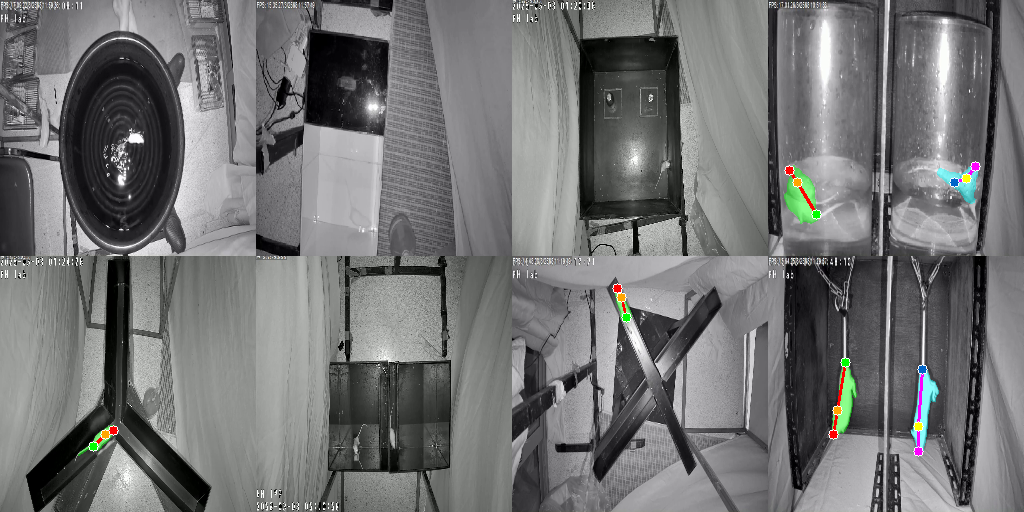
\includegraphics[width=\columnwidth]{figures/qualitative_results.png}
  \caption{Qualitative results across the eight behavioral paradigms.
  Each tile shows HybridMTLNet's per-instance segmentation masks and
  keypoint skeletons (nose--shoulder--tail) on a held-out test image.}
  \label{fig:qualitative}
\end{figure}

\subsection{Single-Task Ablation}
\label{sec:ablation}
To isolate the effect of multi-task learning from architectural
choices, we train the identical HybridMTLNet network in three
configurations on the same data and report each on its relevant
metric (Table~\ref{tab:ablation}). The single-task variants set the
opposing loss weight to zero; the pose-only variant uses heatmap-based
instance matching since its segmentation head is untrained.

\begin{table}[t]
\caption{Single-task ablation on the same network. Joint training
matches single-task segmentation and trades a small amount of pose
accuracy.}
\label{tab:ablation}
\centering
\begin{tabular}{lcc}
\toprule
\textbf{Configuration} & \textbf{mIoU} & \textbf{PCK@0.05} \\
\midrule
Seg-only   & 0.8077 & —      \\
Pose-only  & —      & 0.9791 \\
Joint MTL  & 0.8072 & 0.9552 \\
\bottomrule
\end{tabular}
\end{table}

The ablation shows that joint training does \emph{not} improve either
task: segmentation is essentially unchanged (\(0.8072\) vs.\
\(0.8077\), a \(0.0005\) difference within run-to-run variation),
while pose accuracy decreases slightly (\(0.9552\) vs.\
\(0.9791\), \(-0.024\)). This mild negative transfer on the pose
branch is consistent with known task-interference effects in
multi-task learning \cite{kendall2018multitask, standley2020tasks},
where a shared encoder cannot simultaneously reach the optimum of
each task. We therefore frame the contribution of HybridMTLNet not
as an accuracy gain from joint learning, but as \emph{unification}:
it delivers segmentation and pose at an accuracy comparable to two
dedicated single-task models, while using a single shared encoder,
one forward pass, and fewer parameters.

\subsection{Training Dynamics}
The segmentation loss converges by epoch 30 (mIoU\,\(\approx\)\,0.78),
after which pose PCK continues to improve, reaching 0.9412 on the
validation set by epoch 84. The train/validation gap remains small
throughout (mIoU: 0.031, PCK: 0.019), indicating good generalization
without overfitting.

\subsection{Inference Efficiency}
The principal advantage of HybridMTLNet is efficiency through
unification: both outputs are produced in a single forward pass over
a shared encoder. Table~\ref{tab:efficiency} quantifies this against a
modular alternative that runs two separate single-task models of the
same architecture. At \(256\times256\), HybridMTLNet uses 28.7\,M
parameters and 28.8\,GFLOPs, running at 111.8\,FPS on an RTX~5060 GPU
(14.8\,FPS on CPU). The modular two-model approach doubles every cost
(57.4\,M parameters, 57.5\,GFLOPs, 55.9\,FPS), since it cannot share
encoder computation. HybridMTLNet thus halves memory and compute while
roughly doubling throughput, making it well-suited for real-time
deployment on standard laboratory hardware.

\begin{table}[t]
\caption{Efficiency at \(256\times256\), batch size 1, averaged over
100 runs. The modular baseline runs two separate single-task models.}
\label{tab:efficiency}
\centering
\begin{tabular}{lcccc}
\toprule
\textbf{Approach} & \textbf{Params} & \textbf{FLOPs} & \textbf{GPU} & \textbf{CPU} \\
                  & (M)             & (G)            & (FPS)        & (FPS) \\
\midrule
\textbf{HybridMTLNet} (1 pass) & \textbf{28.7} & \textbf{28.8} & \textbf{111.8} & \textbf{14.8} \\
Modular (2 models)             & 57.4          & 57.5          & 55.9           & 7.4 \\
\bottomrule
\end{tabular}
\end{table}

% ------------------------------------------------------------------
\section{Conclusion}
We presented HybridMTLNet, a multi-task learning framework for
simultaneous instance segmentation and pose estimation of laboratory
mice. By sharing a ResNet-34 encoder between a U-Net segmentation
decoder and a deconvolutional pose head, and by employing Hungarian
matching for order-invariant training, our method outperforms
single-task YOLO26, Mask R-CNN, and DeepLabCut baselines across a
diverse eight-paradigm behavioral dataset. A single-task ablation
shows that this performance is driven by architecture rather than
multi-task synergy: joint training matches single-task segmentation
and incurs only a small pose trade-off, while unifying both tasks in
one model with fewer parameters and a single forward pass. HybridMTLNet
thus provides a practical, unified tool for automated preclinical
behavioral analysis, trading a marginal accuracy cost for substantial
gains in efficiency and deployment simplicity.

\textbf{Limitations and Future Work.}
The current architecture supports a maximum of two mice; extending
to variable instance counts via dynamic slot allocation is a
direction for future work. Additionally, temporal modeling across
video frames could further improve tracking consistency for
behavioral quantification.

% ------------------------------------------------------------------
\section*{Acknowledgment}
[Advisor name and funding acknowledgment here.]

% ------------------------------------------------------------------
\bibliographystyle{IEEEtran}
\bibliography{references}

\end{document}
